\documentclass[a4paper,11pt,oneside,openany]{ltjsbook}
\usepackage[margin=25mm]{geometry}
\usepackage{amsmath,amssymb,booktabs,tabularx,graphicx,xcolor}
\usepackage{tikz}
\usetikzlibrary{arrows.meta,positioning,calc}
\usepackage{listings}
\usepackage{tcolorbox}
\tcbuselibrary{breakable}
\usepackage{xurl}
\usepackage[unicode,hidelinks]{hyperref}
\setlength{\emergencystretch}{2em}
\newcommand{\code}[1]{\nolinkurl{#1}}
\newtcolorbox{goal}{colback=blue!4,colframe=blue!60!black,title=この章で学ぶこと,breakable}
\newtcolorbox{notice}{colback=yellow!5,colframe=orange!80!black,title=注意,breakable}
\lstset{basicstyle=\ttfamily\small,frame=single,backgroundcolor=\color{black!4},breaklines=true,showstringspaces=false,columns=fullflexible}
\tikzset{box/.style={draw,rounded corners,fill=blue!7,align=center,minimum height=10mm,inner sep=5pt}, arrow/.style={-{Stealth},thick}, wire/.style={thick}}
\title{図で理解する kickmix\\[.5em]\large 可逆回路・位相キックバック・軌跡シミュレーション}
\author{Qualtran リポジトリの実装と資料に基づく解説書}
\date{2026年10月}
\begin{document}
\frontmatter\maketitle
\chapter*{本書の読み方}
本書は、Qualtran リポジトリに同梱された \code{kickmix/} のソースコードと \code{docs/kickmix/} の仕様をもとに、量子回路の基礎から使い方、シミュレータの内部構造まで説明する。\code{ref/docs/explanation.tex} の章立て、学習目標、注意欄、TikZ による図解を参考にした。対象読者は線形代数と Python の初歩を知る人である。最初は第1〜4章を順に読み、実際に使う際は第5〜7章を参照してほしい。

\begin{notice}
kickmix は任意の量子回路を状態ベクトルで追跡するシミュレータではない。基底状態上の可逆計算、対角位相、条件付き命令と、制約を満たす測定ベースの逆計算に特化する。後述の HMR の前提を外すと一般の量子力学として正しい結果は得られない。
\end{notice}
\tableofcontents
\mainmatter
\chapter{kickmix の位置づけ}
\begin{goal}何をシミュレートし、何を検証できるかを区別する。\end{goal}
量子アルゴリズムの中には、整数加算、比較、有限体演算などを可逆回路として実行する部分がある。kickmix はそのような部分を小さな命令列に表し、多数の入力や測定結果について、出力と位相を調べる。回路生成・解析と軌跡の実行は分かれた機能である。
\begin{figure}[htbp]\centering
\begin{tikzpicture}[node distance=7mm]
\node[box] (build) {Python の\\CircuitBuilder};
\node[box,right=of build] (circ) {Circuit\\命令列};
\node[box,right=of circ] (sim) {Simulator\\多数の軌跡};
\node[box,below=of circ] (file) {KMX / KMB\\保存・読込};
\node[box,below=of sim] (analysis) {回路図・命令数\\などの解析};
\draw[arrow] (build)--(circ); \draw[arrow] (circ)--(sim); \draw[arrow,<->] (circ)--(file); \draw[arrow] (circ)--(analysis);
\end{tikzpicture}\caption{回路を作る、保存する、実行する、解析するという流れ。}\end{figure}

$ n $ 量子ビットの一般の純粋状態は $2^n$ 個の複素振幅を持つ。一方、kickmix の一軌跡は各量子ビットの計算基底値、古典ビット、および位相を追う。回路が基底状態を別の基底状態へ写し、位相を付ける範囲では、この表現は各入力に対する変換の検査に適する。任意の Hadamard ゲートを含む汎用回路や、干渉のある任意の出力分布を計算する用途には使えない。
\begin{figure}[htbp]\centering
\begin{tikzpicture}[node distance=10mm]
\node[box] (a) {一般の状態ベクトル\\$\sum_x \alpha_x|x\rangle$};
\node[box,right=of a] (b) {kickmix の一軌跡\\$e^{i\theta}|x\rangle$ と古典ビット};
\node[below=3mm of a,align=center] {すべての振幅を保持};
\node[below=3mm of b,align=center] {基底値と位相を保持};
\end{tikzpicture}\caption{内部表現の違い。各軌跡は重ね合わせの全振幅を表すものではない。}\end{figure}

\chapter{基底値と位相の基礎}
\begin{goal}可逆ゲートと対角ゲートが一軌跡に及ぼす変化を追う。\end{goal}
計算基底を $|x\rangle$ とすると、可逆古典回路は $|x\rangle\mapsto|f(x)\rangle$ と書ける。$f$ は置換である。対角ゲートは値を変えず位相を付ける。両者を組み合わせた回路は、測定のない範囲では
\begin{equation}|x\rangle\longmapsto e^{i\theta(x)}|f(x)\rangle\end{equation}
の形で理解できる。入力によって位相が異なると、重ね合わせでは相対位相となり、後段で観測可能な差を生む。
\begin{figure}[htbp]\centering
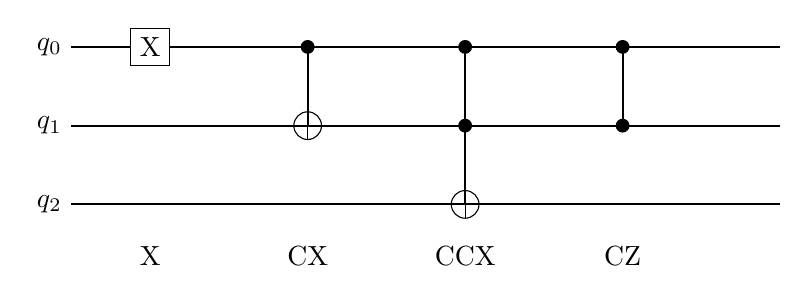
\begin{tikzpicture}[scale=1.0]
\foreach \y/\name in {2/$q_0$,1/$q_1$,0/$q_2$} {\node[left] at (0,\y) {\name}; \draw[wire] (0,\y)--(9,\y);}
\node[draw,fill=white] at (1,2) {X};
\fill (3,2) circle (2.5pt); \draw[wire] (3,2)--(3,1); \draw (3,1) circle (5pt); \draw (2.82,1)--(3.18,1) (3,.82)--(3,1.18);
\fill (5,2) circle (2.5pt); \fill (5,1) circle (2.5pt); \draw[wire] (5,2)--(5,0); \draw (5,0) circle (5pt); \draw (4.82,0)--(5.18,0) (5,-.18)--(5,.18);
\fill (7,2) circle (2.5pt); \fill (7,1) circle (2.5pt); \draw[wire] (7,2)--(7,1);
\node at (1,-.65) {X}; \node at (3,-.65) {CX}; \node at (5,-.65) {CCX}; \node at (7,-.65) {CZ};
\end{tikzpicture}\caption{代表的な命令。黒丸は制御、丸に十字は反転対象。CZ は両方が1のとき位相を反転する。}\end{figure}
具体的には、$\mathrm{CX}: (a,b)\mapsto(a,b\oplus a)$、$\mathrm{CCX}: (a,b,t)\mapsto(a,b,t\oplus ab)$、$\mathrm{CZ}:|a,b\rangle\mapsto(-1)^{ab}|a,b\rangle$ である。\code{Z_POW q0 t} は $|1\rangle$ に $e^{i\pi t}$ を掛ける。一般の $t$ に対して位相は $\pm1$ に限らない。フォーマットは指数を十進数で指定し、通常の倍精度浮動小数点に丸めるだけでは満たせない精度を要求する。

\chapter{HMR と測定ベースの逆計算}
\begin{goal}一時量子ビットを消去する際に生じる位相と補正を導く。\end{goal}
可逆計算では一時値を残すと、入力と補助量子ビットが絡み合う。まず $t=0$ を用意して $t\leftarrow t\oplus ab$ とすると、重ね合わせ入力に対し
\begin{equation}\sum_{a,b} \alpha_{ab}|a,b,0\rangle\longmapsto\sum_{a,b}\alpha_{ab}|a,b,ab\rangle\end{equation}
となる。HMR は対象を X 基底で測定し、結果 $m\in\{0,1\}$ を古典ビットに保存して対象を $|0\rangle$ に戻す。$\langle m_X|t\rangle=(-1)^{mt}/\sqrt2$ より、測定後には $(-1)^{mab}$ が残る。$m=1$ のとき CZ を適用すると同じ符号をもう一度掛けるので消える。
\begin{figure}[htbp]\centering
\begin{tikzpicture}[node distance=6mm]
\node[box] (init) {補助 $t=0$}; \node[box,right=of init] (and) {CCX\\$t=ab$}; \node[box,right=of and] (hmr) {HMR\\$m$, $t=0$}; \node[box,right=of hmr] (fix) {$m=1$ なら CZ\\位相を補正};
\draw[arrow] (init)--(and); \draw[arrow] (and)--(hmr); \draw[arrow] (hmr)--(fix);
\end{tikzpicture}\caption{AND の計算と測定ベースの逆計算。測定値のフィードバックが必要。}\end{figure}
\begin{lstlisting}
R q2
CCX q0 q1 q2
HMR q2 b0
CZ q0 q1 if b0
\end{lstlisting}
\begin{notice}
HMR は対象が他の量子ビットの計算基底値の関数である場合を想定する。この条件を満たさない場合、実装は無作為な結果と位相を使うが、一般の量子状態の正しい測定シミュレーションではない。誤用は位相を含むファズテストで確率的に検出する設計である。\code{R} を非ゼロの値に適用すると位相がランダム化されるため、通常はクリーンな補助量子ビットに使う。
\end{notice}
\code{NEG} は全体符号を反転する。単独の量子状態の全体位相は観測できないが、kickmix は軌跡の位相検査を容易にするため、必要に応じてこの命令による補正も明示する。
\begin{figure}[htbp]\centering
\begin{tikzpicture}[scale=1]
\draw[->] (0,0)--(7,0) node[right] {処理};
\node[box] at (1,1) {$ab=0$\\位相 $+1$};
\node[box] at (3.5,1) {$ab=1,m=1$\\HMR で $-1$};
\node[box] at (6,1) {CZ で再び $-1$\\積は $+1$};
\draw[arrow] (2,1)--(2.5,1);\draw[arrow] (4.5,1)--(5,1);
\end{tikzpicture}\caption{位相補正の例。$m=0$ の場合は補正は不要。}\end{figure}

\chapter{命令とファイル形式}
\begin{goal}KMX の命令、古典制御、レジスタを読む。\end{goal}
KMX は UTF-8 のテキスト形式で、原則として1行に1命令を書く。\code{q} は量子ビット、\code{b} は古典ビット、\code{r} はレジスタの番号を表す。\code{if b0} は量子制御ではなく古典ビットによる実行条件である。
\begin{center}\begin{tabularx}{\textwidth}{lX}\toprule 分類 & 主な命令と役割\\\midrule
量子値の更新 & \code{X}, \code{CX}, \code{CCX}, \code{SWAP}, \code{CSWAP}\\
位相 & \code{Z}, \code{CZ}, \code{CCZ}, \code{Z_POW}, \code{NEG}\\
初期化・測定 & \code{R}, \code{HMR}\\
古典値 & \code{BIT_INVERT}, \code{BIT_STORE0}, \code{BIT_STORE1}\\
条件・メタデータ & \code{PUSH_CONDITION}, \code{POP_CONDITION}, \code{REGISTER}, \code{APPEND_TO_REGISTER}, \code{INFO_TAG}, \code{DEBUG_PRINT}\\\bottomrule\end{tabularx}\end{center}
条件スタックは \code{PUSH_CONDITION if b0} の時点の値を保存する。その後 \code{b0} を書き換えても保存済みの条件は変化しない。通常の命令はスタック上の全条件と、その命令自身の条件が真のときに実行される。条件スタック操作とレジスタ・情報タグのメタデータはスタックを無視する。
\begin{figure}[htbp]\centering
\begin{tikzpicture}[node distance=7mm]
\node[box] (a) {条件なし}; \node[box,right=of a] (b) {push: $b_0$ の値}; \node[box,right=of b] (c) {push: $b_1$ の値}; \node[box,right=of c] (d) {命令を実行\\両方が真のとき};
\draw[arrow] (a)--(b);\draw[arrow] (b)--(c);\draw[arrow] (c)--(d);
\end{tikzpicture}\caption{条件スタックの概念図。pop で直近の条件を取り除く。}\end{figure}
レジスタへの追加順は下位ビットからで、最初の要素が $2^0$ の位を表す。レジスタは名前付きの参照・入出力のためのメタデータであり、宣言自体は量子状態を変えない。
\begin{figure}[htbp]\centering
\begin{tikzpicture}
\foreach \x/\q/\v in {0/q9/$2^0$,2/q6/$2^1$,4/q10/$2^2$} {\draw[fill=blue!8] (\x,0) rectangle +(2,1); \node at (\x+1,.7) {\q}; \node at (\x+1,.3) {\v};}
\node[below] at (3,-.15) {追加順 $\longrightarrow$};
\end{tikzpicture}\caption{リトルエンディアンのレジスタ。量子ビット番号と桁の順序は別である。}\end{figure}
KMB は同じ回路をコンパクトなバイナリで保存する形式である。読み込み・書き出しは \code{Circuit.from_file} と \code{Circuit.to_file} を用いる。詳細な構文、指数の精度、バイナリの符号化は巻末の一次資料を参照する。

\chapter{Python で動かす}
\begin{goal}回路を作り、シミュレータで結果を取得する。\end{goal}
Python 拡張をビルド・インストールした環境で次の例を実行する。\code{Circuit} に KMX テキストを渡し、1ショットの初期値 $q_0=q_9=0$ に対して X と CX を適用する。
\begin{lstlisting}[language=Python]
import kickmix as km

circuit = km.Circuit("""
    X q0
    CX q0 q9
""")
sim = km.Simulator(batch_size=1)
sim.do(circuit)
print(sim.read_within_shot(km.q(0), shot_index=0))  # True
print(sim.read_within_shot(km.q(9), shot_index=0))  # True
\end{lstlisting}
この例では、$00\to10\to11$ と値が変わる。初期値を変えて検査するには \code{write_within_shot} を使う。各ショットの位相は \code{read_shot_phase} で確認できる。測定がある場合は測定結果ごとに補正後の値と位相を検査する。回路だけを用意した段階では何も実行されず、\code{sim.do(circuit)} で初めて状態が変わる。
\begin{figure}[htbp]\centering
\begin{tikzpicture}[node distance=8mm]
\node[box] (c) {Circuit 作成};\node[box,right=of c] (s) {Simulator 作成\\初期値の設定};\node[box,right=of s] (d) {do(circuit)};\node[box,right=of d] (r) {値・位相を読む};
\draw[arrow] (c)--(s);\draw[arrow] (s)--(d);\draw[arrow] (d)--(r);
\end{tikzpicture}\caption{Python API の基本的な実行順序。}\end{figure}
\section{CircuitBuilder と補助量子ビット}
\code{CircuitBuilder} は量子ビットの確保、命令の追加、加算や有限体演算などの回路生成を提供する。慣例上 \code{init_} はクリーンな対象への計算、対応する \code{del_} は逆計算を表す。\code{init_} は対象のリセットを含み、\code{"alloc"} による割り当てをサポートする。これらの前提と確保・解放の寿命を揃えることが重要である。配列を渡した基本ゲートは NumPy に似たブロードキャストを行う。メソッドごとの型と引数は API リファレンスを確認する。

\chapter{シミュレーションの仕組みと検証}
\begin{goal}軌跡の並列処理とテスト結果の意味を理解する。\end{goal}
実装の \code{Sim<TWord, count_shots>} は、各量子ビット・古典ビットについて、複数ショットの値を一つのワードの各ビットに格納する。例えば CX は制御のビット列を対象のビット列に XOR すれば、複数ショットをまとめて更新できる。実際の幅は使用するワード型に依存する。位相には符号のビット列とショットごとの角度が使われる。
\begin{figure}[htbp]\centering
\begin{tikzpicture}
\node[left] at (0,1.4) {$q_0$};\node[left] at (0,.7) {$q_1$};\node[left] at (0,0) {条件};
\foreach \y/\vals in {1.4/{1,0,1,1,0,0,1,0},.7/{0,1,1,0,1,0,0,1},0/{1,1,0,1,0,1,1,0}} {
\foreach \v [count=\i from 0] in \vals {\draw[fill=blue!7] (\i*.8,\y-.3) rectangle +(0.8,.6);\node at (\i*.8+.4,\y) {\v};}}
\node[below] at (3.2,-.45) {列ごとに独立したショット（模式図）};
\end{tikzpicture}\caption{ビットスライス表現。行全体にビット演算を適用する。}\end{figure}
\begin{figure}[htbp]\centering
\begin{tikzpicture}[node distance=9mm]
\node[box] (input) {入力を選ぶ\\またはランダム化};\node[box,right=of input] (run) {回路を実行};\node[box,right=of run] (check) {出力・補助値・\\位相を比較};
\draw[arrow] (input)--(run);\draw[arrow] (run)--(check);
\end{tikzpicture}\caption{典型的な回路検証。出力値だけでなく不要な位相や補助値も確認する。}\end{figure}
入力の全組合せを試せる小規模回路では網羅的な確認が有効である。大規模回路のランダムテストは誤りの発見に役立つが、有限回の成功は正しさの証明ではない。特に HMR の補正漏れは測定結果と入力の組合せによって現れるため、多数の軌跡を使う意味がある。\code{operation_statistics} による命令数の分析と、実行された命令をショットごとに数える分析は別の観点である。

\chapter{再現と資料案内}
\begin{goal}手元でビルドし、詳細仕様と実装をたどる。\end{goal}
リポジトリの開発資料では Bazel 7.2.0、pybind11、pytest を使用し、ルートから次の手順を示している。利用可能なコンパイラ・Python・Bazel 環境に応じて依存関係を整える。
\begin{lstlisting}[language=bash]
bazel build kickmix:kickmix_dev_wheel
pip install bazel-bin/kickmix/kickmix-0.0.dev0-py3-none-any.whl
PYTHONPATH=kickmix pytest kickmix/src
bazel run kickmix:kickmix
\end{lstlisting}
CLI には \code{sample}、\code{diagram}、\code{count_operations}、\code{kmx2kmb}、\code{kmb2kmx} などがある。各サブコマンドのオプションと入出力はソースを確認する。\code{kickmix/testdata/} に KMX と KMB の例がある。
\begin{center}\begin{tabularx}{\textwidth}{lX}\toprule 内容 & リポジトリ内の資料\\\midrule
命令と意味 & \code{docs/kickmix/kickmix_instructions.md}\\
テキスト・バイナリ仕様 & \code{docs/kickmix/kickmix_format.md}, \code{docs/kickmix/kickmix_binary_format.md}\\
Python API と規約 & \code{docs/kickmix/api_reference.md}, \code{docs/kickmix/conventions.md}\\
開発手順 & \code{docs/kickmix/dev.md}\\
軌跡の実装 & \code{kickmix/src/kickmix/sim/sim.h}, \code{sim.cc}\\
使用例と検証 & \code{kickmix/src/kickmix/py/interactive_simulator_test.py} ほか\\
本書の体裁の参考 & \code{ref/docs/explanation.tex}, \code{ref/docs/preamble.tex}\\\bottomrule\end{tabularx}\end{center}
\end{document}
